\par
\subsection{Scenes}
The pie chart below summarizes our results of our work with the scenes data. This chart corresponds to running KNN with n = 5 nearest neighbors (5 was chosen through cross-validation). The labels on the chart give the scene category followed by the percent of correctly predicted labels for that individual scene category. The percentages inside the pie chart correspond to the proportion of times that scene category occurred in our testing sample. 
\begin{figure}[H]
 \centering
 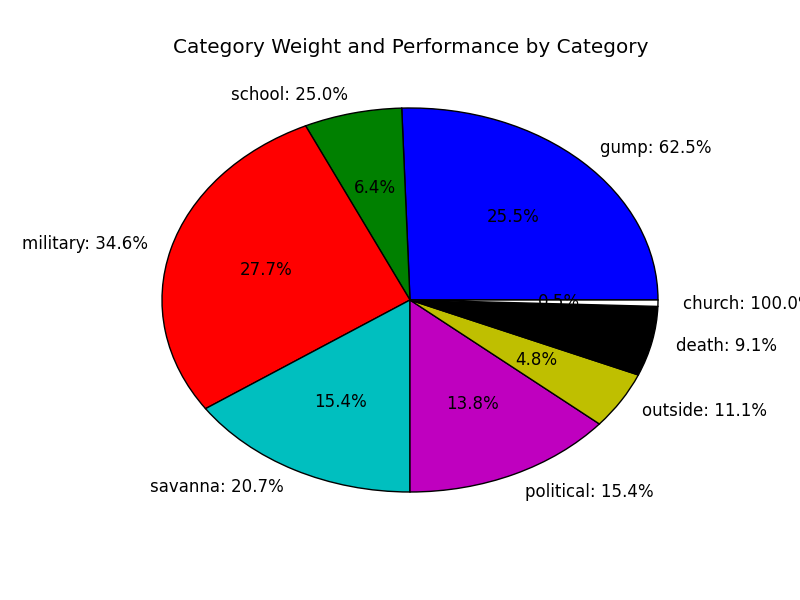
\includegraphics[width=.7\linewidth]{scenes_pie_chart.png}
  \captionof{figure}{KNN performance on the testing sample (total 188 TRs) for each category. Each wedge is proportional to its frequency in the testing sample.}
  \label{fig:test1}
\end{figure}
\par We looked at 8 different categories as specified in the pie chart above. The overall proportion of correctly predicted labels was 34$\%$ but this number, by itself, is not very informative; it does not give us a good idea about the performance with respect to each category and it is skewed by the performance of the more heavily weighted categories. To address this problem, we looked at  how well KNN performed by category and compared this with the relative occurrence of the category. What we see is that for most scenes, KNN performs quite poorly - most hover around the 10$\%$ to 20$\%$ mark. However, the Gump scene seem to be well modeled by KNN with 62$\%$ of its labels correctly matched. It is not clear why the Gump scenes performed better than the others. We initially expected that the Military scenes would be the best as people often react strongly to war. The church scene suggests a good fit with 100$\%$ of the labels correctly matched. However, since there were so few church scenes, this is not very conclusive and could just be a result of random fluctuations.   

\subsection{Ridge Regression}  
The correlation coefficient of the predicted response and the actual response is computed to measure the similarity between the prediction and the actual response for each voxel. The histogram of all correlation coefficients shows that the predicted activity and the actual activity for the majority of the 55468 voxels modeled by ridge regression are highly correlated $(\rho>0.75, p<0.001)$. It shows that the ridge regression model is predicting the brain activity well.
\begin{figure}[H]
 \centering
 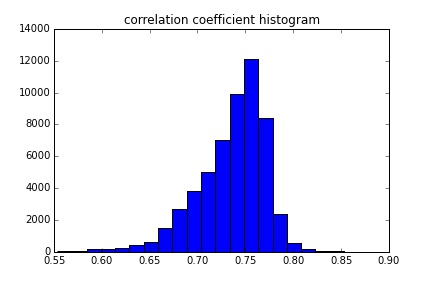
\includegraphics[width=.4\linewidth]{correlation_coefficient_histogram.jpg}
  \captionof{figure}{Correlation coefficients histogram}
  \label{fig:cc}
\end{figure}


\begin{figure}[H]
 \centering
 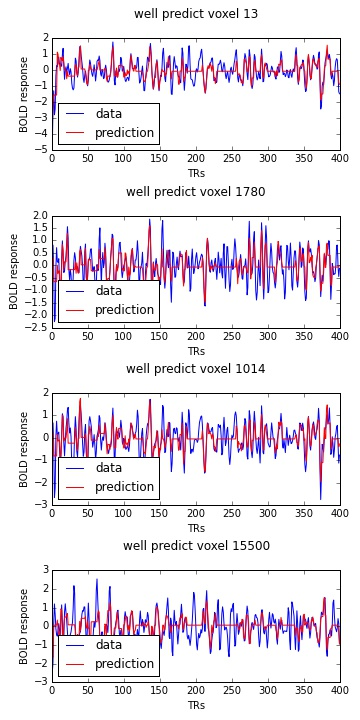
\includegraphics[width=.4\linewidth]{ridge_prediction_results.jpg}
  \captionof{figure}{Examples of voxel predictions}
  \label{fig:test1}
\end{figure}
The figure above shows several examples of predicted activity. The predictions are on around the similar frequency compared to the actual activities, indicating that the model is predicting the activities instead of low frequency noise.

\subsection{Lasso Regression}
\par The lasso regression did not work as well as the ridge regression. As visible from the below plot, the $L1$ prediction is slightly less fitted than the $L2$ regression.

\begin{figure}[H]
 \centering
 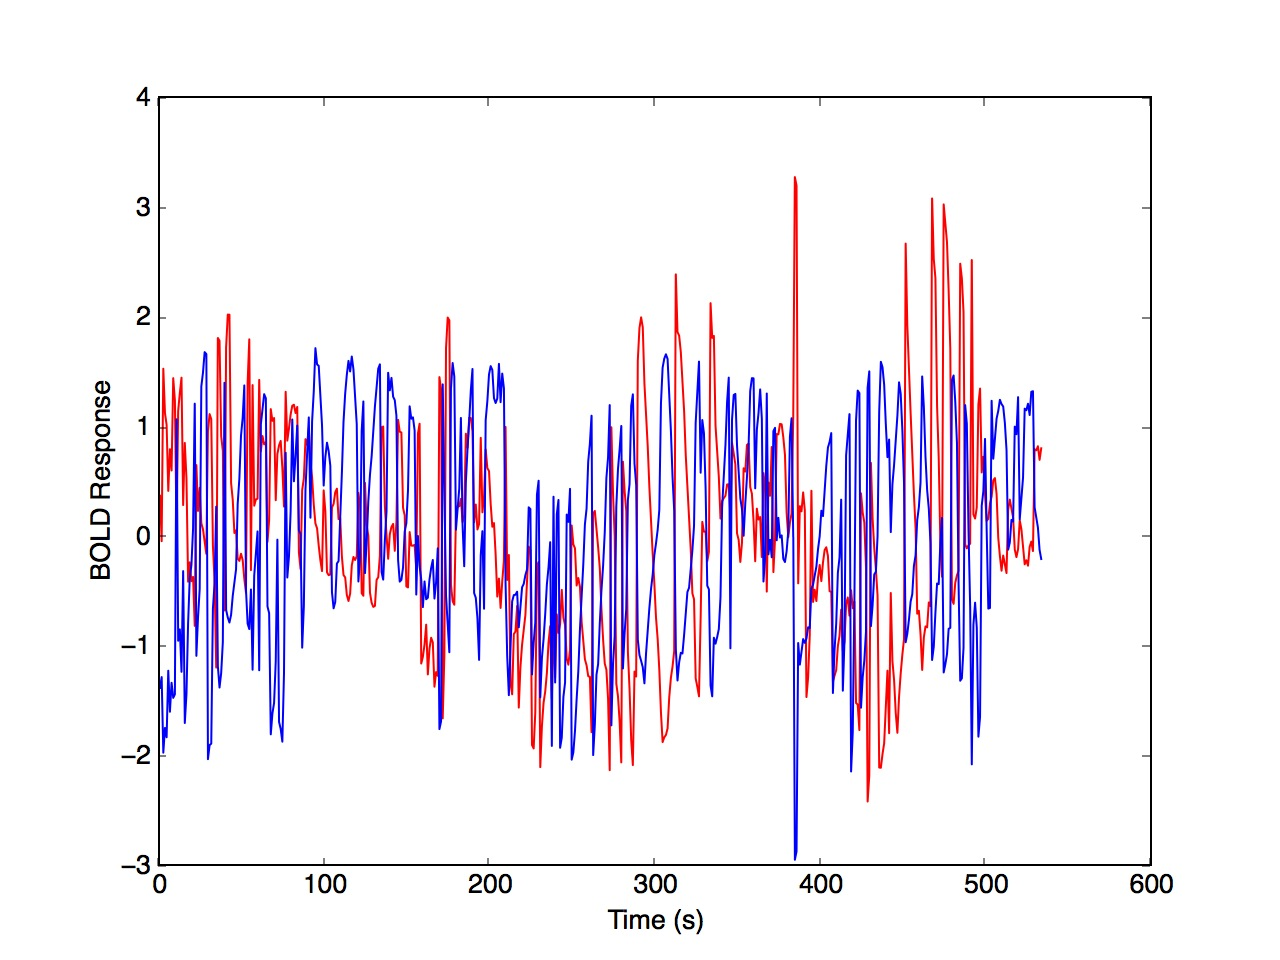
\includegraphics[width=.4\linewidth]{lassoplot.jpg}
  \captionof{figure}{Test Voxel 70 }
  \label{fig:cc}
\end{figure}

\subsection{Neural Network}
\begin{figure}[H]
 \centering
 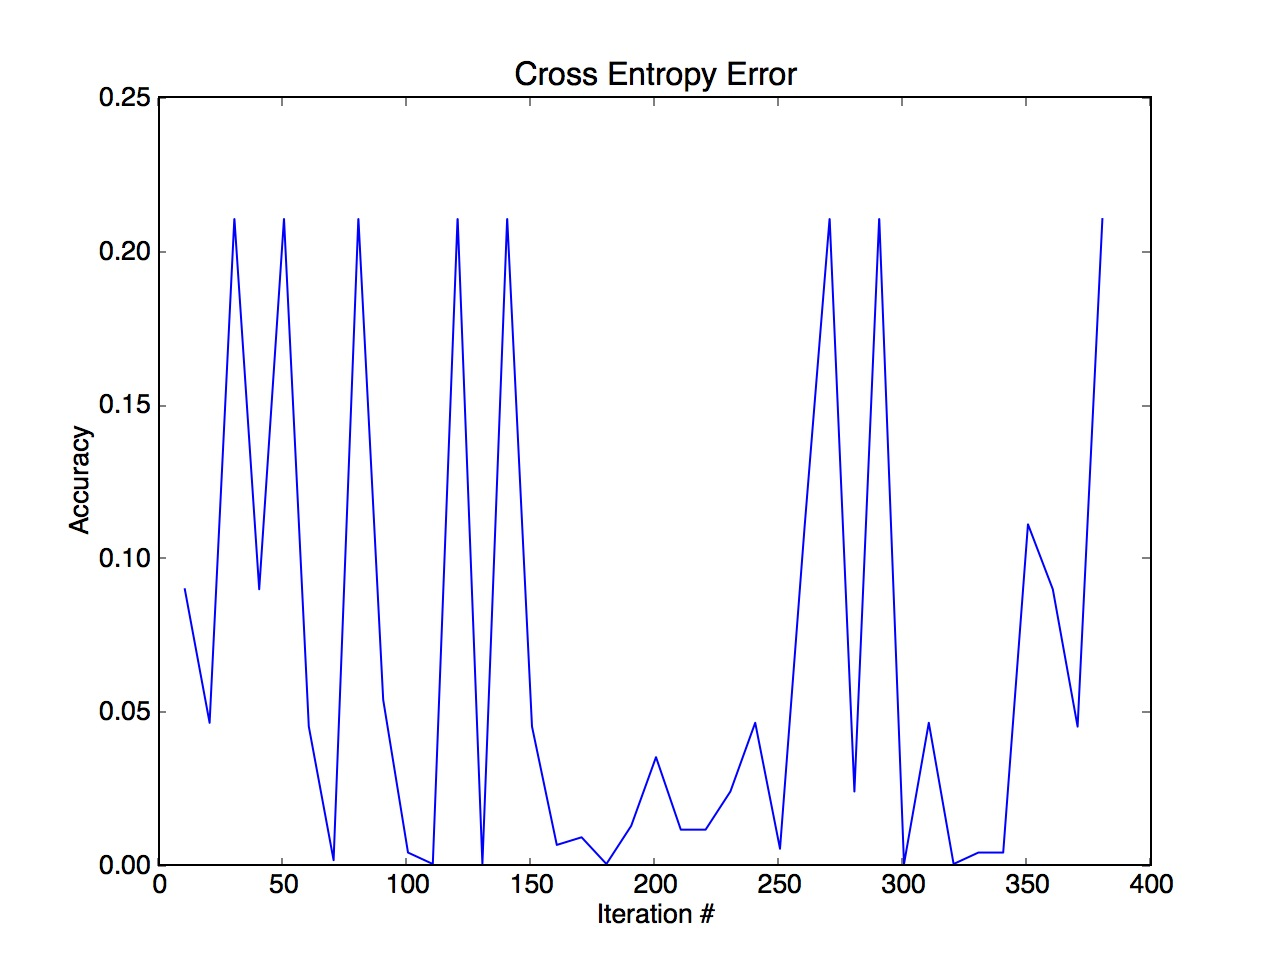
\includegraphics[width=.5\linewidth]{ceallwords.jpg}
  \captionof{figure}{Examples of voxel predictions}
  \label{fig:test1}
\end{figure}

\par The neural network definitely displayed behavior expected of stochastic gradient descent, but was unable to break past 20.099$\%$ accuracy, using the tanh hidden layer activation function. The ReLU activator was very difficult to initialize weights for to get non-zero accuracy, and so was eventually discarded. 

\par Since a correct prediction was defined as correctly predicting the presence/absence of each of the ten words, the by chance predictive accuracy is $\frac{1}{2^{10}}$, or we expect only 1 in 1024 guesses to be correct. The expected accuracy for 300 test points, then, under the assumption that each test point has the same probability of being correct is 
$$E(X) = np = 300\times \frac{1}{2^{10}} \approx .2929  (samples)$$

\par Using a z-test, we can calculate,
$$ Z = \frac{score - \mu}{\sigma} = \frac{18 - .2929}{\sqrt{300\times \frac{1}{1024} \times \frac{1023}{1024}}} \approx 32.7300950233 $$
and from here, 
$$ p = 1 - CDF(Z) \approx 0$$

Thus though there is a generally low probability, at a glance, from the low $p$-value, we can reject a null hypothesis that this is operating by chance and that it's predictions are at least somewhat significant. 















